\chapter{Towards Model-based Run-time State Migration}
\label{ch:requirements}

\section{Requirements Analysis}

A requirement analysis shall be applied to identify what needs to be part of the modeling language and what it should offer.

it's not supporting transition because we don't need to.



\subsection{Same-purpose Applications Analysis}
\subsubsection{States of E-mail Applications}
\begin{table}[ht!]
\begin{tabular}{lll}
State / E-mail client                   & Mailspring & K-9 Mail \\
\hline
Welcome   Screen                        & \checkmark          & \checkmark        \\
Account Registration                    & \checkmark          &          \\
Account Login                           & \checkmark          &          \\
Add an e-mail service account           & \checkmark          & \checkmark        \\
Import   Settings                       &            & \checkmark        \\
Export Settings and Accounts            &            & \checkmark        \\
Settings                                & \checkmark          & \checkmark        \\
Sync New E-mails                        & \checkmark          & \checkmark        \\
Compose a   new E-email                 & \checkmark          & \checkmark        \\
Forward an E-mail                       & \checkmark          &          \\
Replay an   E-mail                      & \checkmark          & \checkmark        \\
Sending an E-mail                       & \checkmark          & \checkmark        \\
Trashing   an E-mail                    & \checkmark          & \checkmark        \\
E-mails list (Inbox, Sent, Draft, …)    & \checkmark          & \checkmark        \\
Single   E-mail                         & \checkmark          & \checkmark        \\
Show Original Version of E-mail         & \checkmark          &          \\
Search   View                           & \checkmark          & \checkmark        \\
Searching                               & \checkmark          & \checkmark        \\
Loading   E-mails                       & \checkmark          & \checkmark        \\
Loading Activity Data                   & \checkmark          &          \\
Activity   View                         & \checkmark          &          \\
Exporting Activity Data                 & \checkmark          &          \\
Sharing   Report of Activity Data       & \checkmark          &          \\
Marking Star/Spam/Read/Unread an E-mail & \checkmark          & \checkmark       
\end{tabular}
\caption{States of E-mail Applications}
\label{tab:states_of_email_applications}
\end{table}

\newpage
\subsubsection{States of Browsers}

Chrome Page lifecycle API
https://developers.google.com/web/updates/2018/07/page-lifecycle-api

W3C Page lifecycle API
https://wicg.github.io/page-lifecycle/

Mozilla Web API
https://developer.mozilla.org/en-US/docs/Web/API


\begin{table}[ht!]
\begin{tabular}{lll}
State / Browser                                       & Firefox (macOS) & Chrome (Android) \\
\hline
Home page                                             & \checkmark      & \checkmark       \\
Single Tab (Preferences, Bookmarks, Performance,   …) & \checkmark      & \checkmark       \\
Extensions   Tab                                      & \checkmark      &                  \\
Syncing                                               & \checkmark      & \checkmark       \\
Browsing                                              & \checkmark      & \checkmark       \\
Current Tab                                           & \checkmark      & \checkmark       \\
Developer   Console                                   & \checkmark      &                  \\
Signing in                                            & \checkmark      & \checkmark       \\
Finding   (in page)                                   & \checkmark      & \checkmark       \\
Printing                                              & \checkmark      &                  \\
Downloading                                           & \checkmark      & \checkmark       \\
Sharing                                               &                 & \checkmark       \\
Private/Incognito   Mode                              & \checkmark      & \checkmark       \\
Light mode                                            &                 & \checkmark      
\end{tabular}
\caption{States of Browsers applications}
\label{tab:state_browsers}
\end{table}


\subsubsection{States of Video Player Applications}
For migration of video players, we needed to access to video file, considering the run-time migration of video players is not a good choice.

\begin{table}[ht!]
\begin{tabular}{lll}
State / Video Player                                               & IINA (macOS) & VLC (Android) \\
\hline
Welcome   Screen                                                   & \checkmark       & \checkmark        \\
Video player tips                                                  &              & \checkmark        \\
Audio   player tips                                                &              & \checkmark        \\
Pause                                                              & \checkmark       & \checkmark        \\
Deleting                                                           &              & \checkmark        \\
Browsing view                                                      & \checkmark       & \checkmark        \\
Loading   Directories                                              &              & \checkmark        \\
Single Page view (About, Settings, Audio,   Video, …) & \checkmark       & \checkmark        \\
Search   result                                                    &              & \checkmark        \\
Searching                                                          &              & \checkmark        \\
Playing   video                                                    & \checkmark       & \checkmark        \\
Playing audio                                                      & \checkmark       &               \\
Showing   picture                                                  & \checkmark       &               \\
Streaming                                                          & \checkmark       & \checkmark        \\
Loading   local network devices                                    &              & \checkmark       
\end{tabular}
\caption{States of Video player applications}
\label{tab:states_video_players}
\end{table}

\newpage
\subsubsection{States of Note Taking Applications}

\begin{table}[ht!]
\begin{tabular}{lll}
State / Note taking application                                          & Laverna (macOS) & Joplin (Android) \\
\hline
Loading   Screen                                                         & \checkmark          &                  \\
Welcome Screen                                                           & \checkmark          &                  \\
Encryption   view                                                        & \checkmark          &                  \\
Syncing on Cloud                                                         & \checkmark          & \checkmark           \\
Importing   and Exporting settings                                       & \checkmark          &                  \\
Importing and Exporting data                                             & \checkmark          & \checkmark           \\
Single   Page view (All notes, Favorites, Settings, ...) & \checkmark          & \checkmark           \\
Search                                                                   & \checkmark          & \checkmark           \\
Searching                                                                & \checkmark          & \checkmark           \\
Writing a Note                                                           & \checkmark          & \checkmark           \\
Writing a   Todo                                                         &                 & \checkmark           \\
Saving a Note                                                            & \checkmark          & \checkmark           \\
Note   Properties                                                        &                 & \checkmark           \\
New Notebook                                                             & \checkmark          & \checkmark           \\
New Tags                                                                 & \checkmark          & \checkmark           \\
Share view                                                               &                 & \checkmark           \\
Trashing                                                                 & \checkmark          &                  \\
Removing                                                                 & \checkmark          &                 
\end{tabular}
\caption{States of Note taking applications}
\label{tab:states_note_apps}
\end{table}

\newpage
\subsubsection{Modeling States of E-mail Applications}

\begin{table}[ht!]
\begin{tabular}{lll}
Field     & Type      & Example/Description                                    \\
\hline
id        & String/Id & pYkSAMPpfU9bU1E33219fbaJyVoQ71hS8Vvs7gDZC              \\
aid       & String/Id & 0a6dbf86                                               \\
v         & Number    & 3                                                      \\
metadata  & Array     & Information   About Mail/Link tracking                 \\
to        & Array     & []                                                     \\
cc        & Array     & []                                                     \\
bcc       & Array     & []                                                     \\
from      & Array     & []                                                     \\
replyto   & Array     & []                                                     \\
date      & Number    & 1595782508                                             \\
body      & String    & <div>This is a test   body</div><br/>                  \\
files     & Array     & []                                                     \\
unread    & Boolean   & False                                                  \\
events    & Array     & []                                                     \\
starred   & Boolean   & False                                                  \\
threadid  & String/Id & “”                                                     \\
subject   & String    & Test   Subject                                         \\
draft     & Boolean   & True                                                   \\
pristine  & Boolean   & False                                                  \\
plaintext & Boolean   & False                                                  \\
folder    & Object    & {}                                                     \\
"file\_ids"  & Array  & []                                                  \\
object    & String    & “draft”                                               
\end{tabular}
\caption{Modeling the State: Compose a new Email in Mailspring}
\label{tab:compose_new_email_mailspring}
\end{table}


\newpage
\begin{table}[ht!]
\begin{tabular}{lll}
Field     & Type      & Example/Description \\
\hline
\_ID            &  &  \\
SEND\_DATE      &      &                     \\
SENDER         &      &                     \\
SUBJECT        &      &                     \\
PREVIEW        &      &                     \\
ACCOUNT        &      &                     \\
DELETE\_URI     &      &                     \\
SENDER\_ADDRESS &      &                    
\end{tabular}
\caption{Modeling the State: Compose a new Email in K-9 Mail}
\label{tab:compose_new_email_k9}
\end{table}


\begin{table}[ht!]
\begin{tabular}{lll}
Field       & Type    & Example/Description \\
\hline
isSearching & Boolean & False               \\
query       & String  & “master   thesis”  
\end{tabular}
\caption{Modeling the State: Search in Mailspring}
\label{tab:search_mailspring}
\end{table}


\begin{table}[ht!]
\begin{tabular}{lll}
Field & Type   & Example/Description \\
\hline
query & String & “master thesis”    
\end{tabular}
\caption{Modeling the State: Search in K-9 Mail}
\label{tab:search-k9}
\end{table}

\section{Solution Overview}
a model-driven approach, as outlined in Figure \ref{fig:solution}, shall be developed. 

\begin{figure}[!b]
    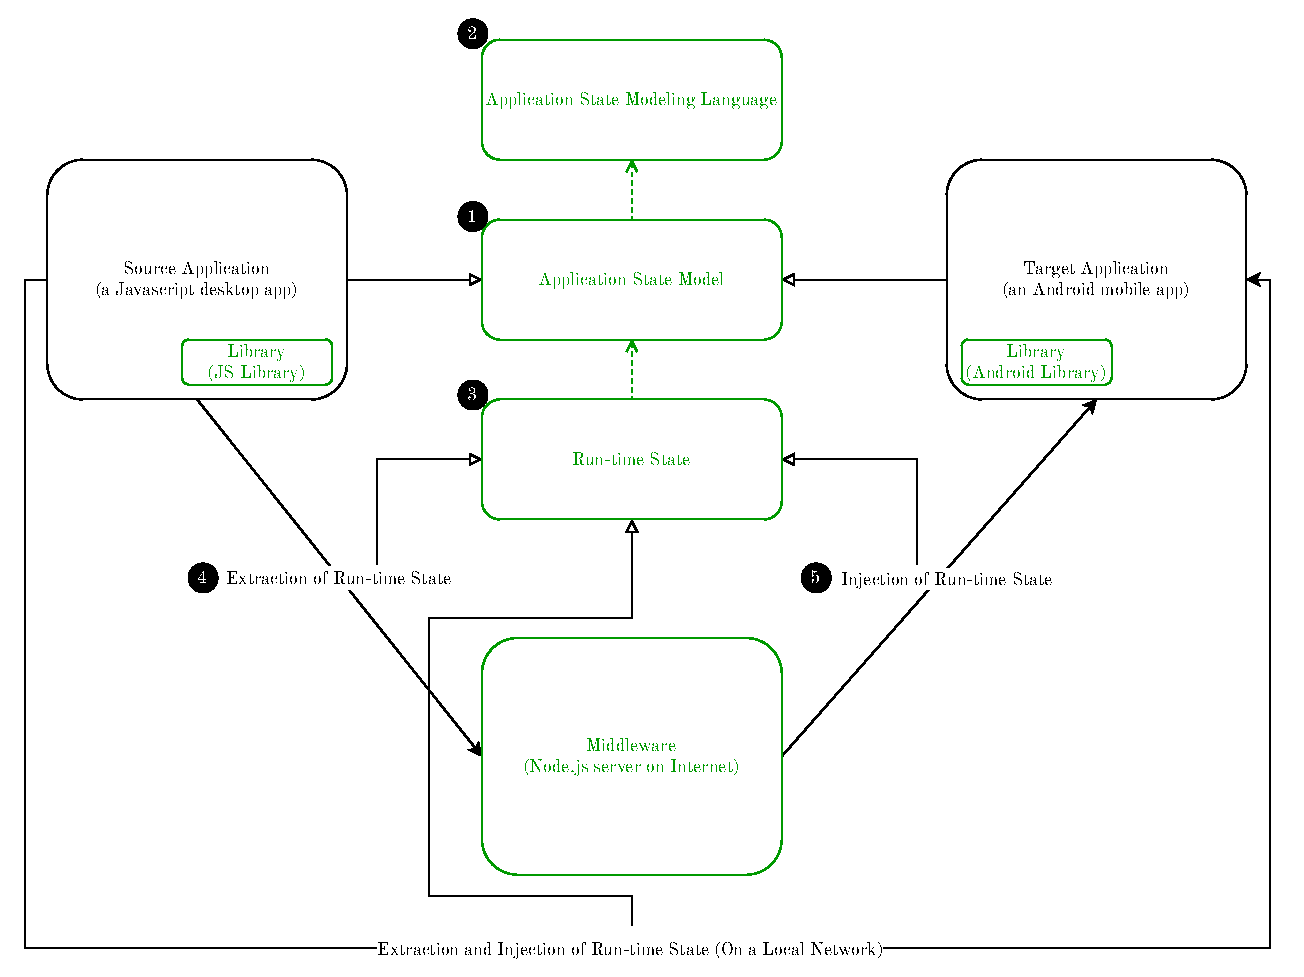
\includepdf[width=\linewidth, offset= 0 -100]{../figures/solution.pdf}
    % \vspace{10cm}
    \caption{Showing the approach of run-time state migration between two applications }
    \label{fig:solution}
\end{figure}

\newpage